\begin{center}
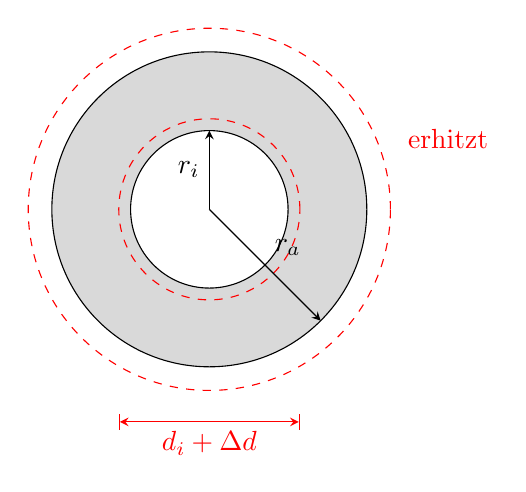
\begin{tikzpicture}[>=stealth]
 \fill[gray!30, even odd rule] (0,0) circle (2.0) (0,0) circle (1.0);
 \draw (0,0) circle (2.0);
 \draw (0,0) circle (1.0);
 \draw[red, dashed] (0,0) circle (2.3);
 \draw[red, dashed] (0,0) circle (1.15);
 \draw[->] (0,0) -- (0,1.0) node[midway, left] {$r_i$};
 \draw[->] (0,0) -- (1.414,-1.414) node[midway, above right] {$r_a$};
 \draw[red, |<->|] (-1.15,-2.7) -- (1.15,-2.7) node[midway, below] {$d_i+\Delta d$};
 \node[red, anchor=west] at (2.4,0.9) {erhitzt};
\end{tikzpicture}
\end{center}

Beim Erhitzen dehnt sich das Metall in alle Richtungen gleichmässig aus: Jede Strecke im Ring wird um denselben Faktor $1+\alpha\,\Delta\vartheta$ länger. Der Ring wird also wie bei einer fotografischen Vergrösserung als Ganzes ähnlich vergrössert. Das gilt auch für den Innenrand: Sein Umfang $2\pi r_i$ besteht aus Metall und wird länger, also wird auch das Loch grösser, nicht kleiner. Der neue Innenradius ist
\begin{align}
 r_i' &= r_i\left(1+\alpha\,\Delta\vartheta\right)
\end{align}
und der Lochdurchmesser ändert sich um
\begin{align}
 \Delta d &= 2\,r_i' - 2\,r_i = \result{2\,r_i\,\alpha\,\Delta\vartheta}
\end{align}
Das Loch dehnt sich genau so aus, als wäre es mit dem Metall des Rings gefüllt. Die Änderung hängt nicht vom Aussenradius $r_a$ ab.
